\documentclass[a4paper]{report}
\usepackage[utf8]{inputenc}
\usepackage{hyperref}
\usepackage{a4wide}
\hypersetup{pdftitle={Key Value Store},
pdfauthor={João Teixeira, José Ferreira},
colorlinks=true,
urlcolor=blue,
linkcolor=black}
\usepackage{subcaption}
\usepackage[cache=false]{minted}
\usepackage{listings}
\usepackage{booktabs}
\usepackage{multirow}
\usepackage{appendix}
\usepackage{tikz}
\usepackage{authblk}
\usepackage{bashful}
\usepackage{verbatim}
\usepackage{amssymb}
\usepackage{multirow}
\usepackage{mwe}
\usepackage[parfill]{parskip}
\usetikzlibrary{positioning,automata,decorations.markings}
\AfterEndEnvironment{figure}{\noindent\ignorespaces}
\AfterEndEnvironment{table}{\noindent\ignorespaces}

\usepackage{titlesec}

\titleformat{\chapter}[display]
   {\normalfont\large\bfseries}{\chaptertitlename\ \thechapter}{0pt}{\huge}
\titlespacing*{\chapter}{0pt}{0pt}{0pt}

\begin{document}

\title{Algoritmos Paralelos\\Stencil2D e All-Pairs Shortest Paths}
\author{João Teixeira (A85504) \and José Filipe Ferreira (A83683)}
\date{\today}

\begin{center}
    \begin{minipage}{0.75\linewidth}
        \centering
        
\includegraphics[width=0.4\textwidth]{images/eng.jpeg}\par\vspace{1cm}
        \vspace{1.5cm}
        \href{https://www.uminho.pt/PT}
        {\color{black}{\scshape\LARGE Universidade do Minho}} \par
        \vspace{1cm}
        \href{https://www.di.uminho.pt/}
        {\color{black}{\scshape\Large Departamento de Informática}} \par
        \vspace{1.5cm}
        \maketitle
    \end{minipage}
\end{center}

\tableofcontents

\chapter{Introdução}

O objetivo deste trabalho pratico é escolher dois algoritmos e analisar a sua
escalabilidade. Os algoritmos escolhidos para este propósito foram o
\textit{All-Pairs Shortest Path} e o \textit{Stencil2D}.

Ao longo deste relatório iremos descrever os passos tomados para fazer esta
analise. Começando por descrever como foi desenvolvida a versão sequencial do
algoritmo, em seguida descrevendo como foi criada a versão paralela e por fim
comparando a performance das duas.

Todos os testes de performance foram realizados no cluster SeARCH da
Universidade do Minho nas maquinas 641 com dual Intel Xeon E5-2650v2 a 2.60GHz e
64GiB de memória RAM. Para cada valor foram retiradas cinco medidas distintas e é
apresentada a mediana dessas cinco medições. Uma tabela com todas as medições
está disponível no Apêndice \ref{ch:medicoes}.

\chapter{Stencil2D}

O algoritmo Stencil2D é um algoritmo que consiste em criar múltiplas iterações
sobre uma dada matriz. No inicio de cada iteração percorre-se cada ponto da
matriz, excluindo os pontos na moldura exterior, e cria-se uma matriz nova em
que cada ponto corresponde à media entre os pontos a norte, sul, este e oeste da
matriz da iteração anterior (Imagem \ref{fig:stencil2dit}). Desta forma, cada
iteração tem complexidade O(n²) sendo n o tamanho da matriz.


\begin{verbatim}
Begin
  for it := 0 to IT, do
    for i := 1 to N-1, do
      for j := 1 to N-1, do
         G1[i,j] = 0.2 * (G2[i-1,j] + G2[i+1,j] + G2[i,j-1] + G2[i,j+1] + G2[i,j]);
      done
    done
    copy(G1,G2)
  done
End
\end{verbatim}

\begin{figure}[h]
    \centering
        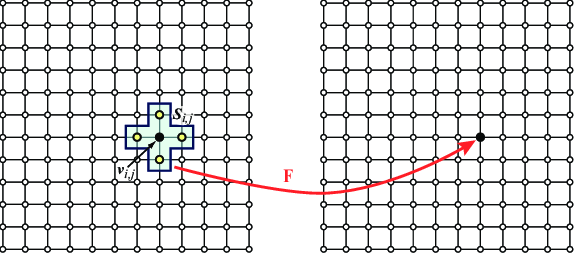
\includegraphics[width=0.5\textwidth]{images/2D-example-of-stencil-computation.png}
        \caption{representação de uma iteração do algoritmo}
        \label{fig:stencil2dit}
\end{figure}

Numa primeira versão da implementação deste algoritmo copiamos no fim de cada
iteração a matriz onde se esta a escrever para uma matriz auxiliar que guarda a
iteração anterior fazendo uso da função \textit{memcpy}. Esta copia é
extremamente lenta e pode ser optimizada.

Inspirados na forma como uma placa gráfica lida com buffers para renderizar
imagens decidimos, em vez de copiar a matriz para uma matriz auxiliar, alternar
a matriz onde se escreve e a matriz onde se lê em cada iteração. Desta forma
evitam-se as copias de matriz e melhora-se a performance.

Com o objetivo de paralelizar esta última versão desenvolvida decidimos analisar
o \textit{vectorization report} criado pelo gcc. Desta forma constatamos que o
loop que percorre ao longo de cada linha da matriz (o loop mais interior)
vectoriza (Imagem \ref{fig:stencil2dgcc}) e, por isso, paralelizar este loop, em
principio, seria
contraproducente. Por outro lado, o loop exterior referente às iterações tem
dependência de dados entre cada uma. Desta forma resta o loop referente a
percorrer todas as linhas para ser vetorizado.

\begin{figure}[h]
    \centering
        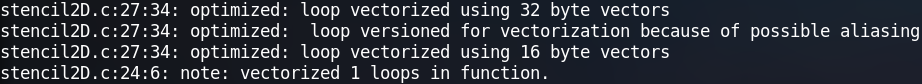
\includegraphics[width=0.7\textwidth]{images/stencil2D_gcc.png}
        \caption{excerto do Vectorization Report no GCC}
        \label{fig:stencil2dgcc}
\end{figure}

\begin{table}[h]
\centering
\begin{tabular}{|l|c|c|c|}
\hline
Versão & \multicolumn{1}{l|}{OpenMP threads} & \multicolumn{1}{l|}{tempo (s)} & \multicolumn{1}{l|}{speedup} \\ \hline
stencil2D sequencial & -  & 17.703 & - \\ \hline
stencil2D sequencial sem copias & -  & 7.004  & 2.528 \\ \hline
\multirow{2}{*}{stencil2D paralelizado sem copias} & 16 & 4.39 & 4.033 \\ \cline{2-4}
                     & 32 & 1.835  & 9.647 \\ \hline
\end{tabular}
\caption{tempos e speedup para stencil2D}
\label{tab:stencil2Dtimes}
\end{table}

\chapter{All-Pairs Shortest Path}

O algoritmo \textit{All-Pairs Shortest Path} consiste em percorrer um grafo
orientado pesado representado sobre a forma de uma matriz N por N,sendo N o
número de vértices no grafo, em que o valor de cada
posição (i,j) representa o custo da aresta que vai do nodo i para o nodo j. No fim deste
algoritmo correr, em cada posição (i,j) estará presente o custo mínimo de ir do
nodo i para o nodo j.

\begin{verbatim}
Begin
  for k := 0 to N, do
    for i := 0 to N, do
      for j := 0 to N, do
        if cost[i,k] + cost[k,j] < cost[i,j], then
          cost[i,j] := cost[i,k] + cost[k,j]
        done
      done
  done
End
\end{verbatim}

Primeiro analisamos o código disponibilizado. Com base no \textit{vectorization
report} disponibilizado pelo gcc constatamos que o loop mais interior vetoriza
quando se aplica a flag -O3 no compilador (Imagem \ref{fig:aspgcc}).
Por isso, paralelizar este loop seria contra produtivo.

\begin{figure}[h]
    \centering
        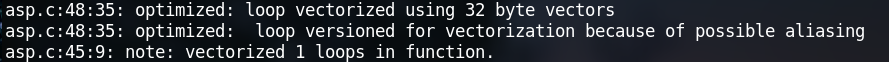
\includegraphics[width=0.8\textwidth]{images/asp_gcc.png}
        \caption{excerto do Vectorization Report do GCC}
        \label{fig:aspgcc}
\end{figure}

Com o objetivo de analisar qual dos dois loops restantes é o melhor para
paralelizar foram criadas duas versões distintas da função. Analisando os
resultados presentes na tabela \ref{tab:asptimes} constatamos que é mais vantajoso paralelizar o
loop exterior (neste caso o loop com a variável k).

Após analisarmos como a matriz é percorrida constatamos que a matriz é
percorrida coluna por coluna. Desta forma as colisões na cache são maiores. Se
trocarmos a ordem dos dois loops exteriores este problema fica resolvido. Para
tentar extrair ainda mais performance decidimos alinhar a matriz, diminuindo
assim ainda mais as colisões na cache do CPU.

\begin{verbatim}
int cost[N][N]__attribute__((aligned (32)));
\end{verbatim}

\begin{table}[h]
\centering
\begin{tabular}{|l|c|c|c|}
\hline
Versão & \multicolumn{1}{l|}{OpenMP threads} & \multicolumn{1}{l|}{tempo (s)} & \multicolumn{1}{l|}{speedup} \\ \hline
asp sequencial & -  & 6.825 & - \\ \hline
\multirow{2}{*}{asp paralelo i} & 16 & 1.695 & 4.027 \\ \cline{2-4}
                                & 32 & 0.904  & 7.550 \\ \hline
\multirow{2}{*}{asp paralelo k} & 16 & 1.124 & 6.072 \\ \cline{2-4}
                                & 32 & 0.638  & 10.697 \\ \hline
\multirow{2}{*}{asp swap paralelo alinhado} & 16 & 1.147 & 5.950 \\ \cline{2-4}
                                            & 32 & 0.596  & 11.451 \\ \hline
\end{tabular}
\caption{tempos e speedup para stencil2D}
\label{tab:asptimes}
\end{table}

\appendix

\chapter{Medições Realizadas}
\label{ch:medicoes}

\begin{table}[h]
\centering
\begin{tabular}{|l|l|c|c|c|c|c|c|c|}
\hline
Algoritmo &
  Versão &
  \multicolumn{1}{l|}{n threads} &
  \multicolumn{1}{l|}{teste 1} &
  \multicolumn{1}{l|}{teste 2} &
  \multicolumn{1}{l|}{teste 3} &
  \multicolumn{1}{l|}{teste 4} &
  \multicolumn{1}{l|}{teste 5} &
  \multicolumn{1}{l|}{mediana} \\ \hline
\multirow{4}{*}{Stencil2D} & com copias                              & -  & 17.220 & 16.901 & 21.043 & 17.703 & 19.520 & 17.703 \\ \cline{2-9}
                           & sem copias                              & -  & 6.779  & 7.004  & 7.010  & 6.811  & 7.074  & 7.004  \\ \cline{2-9}
                           & \multirow{2}{*}{paralelo sem copias}    & 16 & 4.390  & 4.425  & 4.410  & 4.040  & 4.221  & 4.390  \\ \cline{3-9}
                           &                                         & 32 & 1.842  & 1.778  & 1.835  & 1.854  & 1.787  & 1.835  \\ \hline
\multirow{7}{*}{ASP}       & sequencial                              & -  & 7.492  & 6.824  & 7.308  & 6.753  & 6.825  & 6.825  \\ \cline{2-9}
                           & \multirow{2}{*}{paralelo k}             & 16 & 0.972  & 1.133  & 0.939  & 1.124  & 1.291  & 1.124  \\ \cline{3-9}
                           &                                         & 32 & 0.842  & 0.628  & 0.616  & 0.638  & 0.663  & 0.638  \\ \cline{2-9}
                           & \multirow{2}{*}{paralelo i}             & 16 & 1.733  & 1.636  & 1.695  & 2.190  & 1.660  & 1.695  \\ \cline{3-9}
                           &                                         & 32 & 0.904  & 0.914  & 1.235  & 0.884  & 0.886  & 0.904  \\ \cline{2-9}
                           & \multirow{2}{*}{swap paralelo alinhado} & 16 & 1.119  & 1.147  & 1.153  & 1.160  & 1.162  & 1.147  \\ \cline{3-9}
                           &                                         & 32 & 0.574  & 0.595  & 0.598  & 0.664  & 0.594  & 0.595  \\ \hline
\end{tabular}
\caption{Medições realizadas}
\label{tab:medicoes}
\end{table}

\end{document}
